\documentclass[12pt,twoside]{article}
%\date{}   %uncommenting this erases the date
\usepackage{graphicx}
\usepackage{amsmath}
\usepackage{amssymb}
\usepackage{natbib}
\usepackage{verbatim}
\usepackage{floatpag}
\usepackage{subeqnarray}
\usepackage{mathrsfs}    %for special characters
\usepackage{cancel}  % to set terms in an equation to zero


\setlength{\textheight}     {9.0in}
\setlength{\textwidth}      {6.5in}
\setlength{\oddsidemargin}  {0.0in}
\setlength{\evensidemargin} {0.0in}
\setlength{\topmargin}      {0.0in}
\setlength{\headheight}     {0.0in}
\setlength{\headsep}        {0.0in}
\setlength{\hoffset}        {0.0in}
\setlength{\voffset}        {0.0in}
\setlength{\parindent}      {0.0in}      %starting new line at extreme left

\graphicspath{{Figures/}}

\newcommand{\astrut}{\usebox{\astrutbox}}

\newcommand\GaPQ{\ensuremath{G_a(P,Q)}}
\newcommand\GsPQ{\ensuremath{G_s(P,Q)}}
\newcommand\p{\ensuremath{\partial}}
\newcommand\tti{\ensuremath{\rightarrow\infty}}
\newcommand\kgd{\ensuremath{k\gamma d}}
\newcommand\shalf{\ensuremath{{\scriptstyle\frac{1}{2}}}}
\newcommand\sh{\ensuremath{^{\shalf}}}
\newcommand\smh{\ensuremath{^{-\shalf}}}
\newcommand\squart{\ensuremath{{\textstyle\frac{1}{4}}}}
\newcommand\thalf{\ensuremath{{\textstyle\frac{1}{2}}}}
\newcommand\Gat{\ensuremath{\widetilde{G_a}}}
\newcommand\ttz{\ensuremath{\rightarrow 0}}
\newcommand\ndq{\ensuremath{\frac{\mbox{$\partial$}}{\mbox{$\partial$} n_q}}}
\newcommand\sumjm{\ensuremath{\sum_{j=1}^{M}}}
\newcommand\pvi{\ensuremath{\int_0^{\infty}%
  \mskip \ifCUPmtlplainloaded -30mu\else -33mu\fi -\quad}}

\newcommand\etal{\mbox{\textit{et al.}}}
\newcommand\etc{etc.\ }
\newcommand\eg{e.g.\ }



\newcommand{\bs}  [1]{\boldsymbol{#1}}
\newcommand{\del} {\nabla}
\newcommand{\bsh}  [1]{\boldsymbol{\hat{#1}}}
\newcommand{\ul}  {\underline}
\newcommand{\ol}  {\overline}
\newcommand{\pp} [2]{\frac{\p{#1}}{\p{#2}}}
\newcommand{\dd} [2]{\frac{d{#1}}{d{#2}}}
\newcommand{\lam}  [1]{{#1}^{\tiny{\lambda}}}
\newcommand{\conj} [1]{{#1}^*}
\newcommand{\mods} [1]{ \vert {#1} \vert ^2}

\newcommand{\ph} [1]{ \langle #1 \rangle }  % For phase shorthand

\newcommand{\bsp} [1]{ \bs { #1^{\perp} }  }  % For phase shorthand

\newcommand{\w} [1]{  { {#1}_{\scriptscriptstyle W} }  }  % For wave shorthand

\newcommand{\g} [1]{  { {#1}_{\scriptscriptstyle G} }  }  % For geostrophic shorthand

\newcommand{\io} [1]{  { {#1}_{\scriptscriptstyle {IO} } }  }  % For io shorthand

\newcommand{\iw} [1]{  { {#1}_{\scriptscriptstyle {IW} } }  }  % For io shorthand

\newcommand{\spc}[1] {\mathscr {#1} }

%%% short hands for two waves and geostrophic modes %%%

\newcommand{\wf} [1]{  { {#1}_{\scriptscriptstyle {W1} } }  }  % For wave 1 shorthand

\newcommand{\wfc} [1]{  { {#1}^*_{\scriptscriptstyle {W1} } }  }  % For wave 1 c.c. shorthand

\newcommand{\ws} [1]{  { {#1}_{\scriptscriptstyle {W2} } }  }  % For wave 2 shorthand

\newcommand{\wsc} [1]{  { {#1}^*_{\scriptscriptstyle {W2} } }  }  % For wave 2 c.c. shorthand

\newcommand{\gf} [1]{  { {#1}_{\scriptscriptstyle {G1} } }  }  % For geostrophic 1 shorthand

\newcommand{\gfc} [1]{  { {#1}^*_{\scriptscriptstyle {G1} } }  }  % For geostrophic 1 c.c shorthand

\newcommand{\gfsq} [1]{  { {#1}^2_{\scriptscriptstyle {G1} } }  }  % For geostrophic 1 squared shorthand

\newcommand{\gs} [1]{  { {#1}_{\scriptscriptstyle {G2} } }  }  % For geostrophic 2 shorthand

\newcommand{\gsc} [1]{  { {#1}^*_{\scriptscriptstyle {G2} } }  }  % For geostrophic 2 c.c shorthand

\newcommand{\gssq} [1]{  { {#1}^2_{\scriptscriptstyle {G2} } }  }  % For geostrophic 2 squared shorthand

%%% short hands for two waves and geostrophic modes %%%

\title{Investigation into singularity formation in the Birkhoff-Rott Equation }

\author{Raghav Singhal}

\begin{document}
\maketitle

In this work we have computed the curvature, $x_{\Gamma \Gamma} ,        y_{\Gamma \Gamma}$ and the solution of our model . We trace the maximum and minimum point of the curvature in the solution and observe how that corresponds to the sharpening of the inner and outer curves, once we move past the critical time (experimentally determined  $t_c=0.54$). We also noticed that maximum and minimum points of the curbature move towards each other but once past the critical time, it doesn't fluctuate a lot.
\begin{figure}[ht]
\centering
\begin{minipage}[b]{0.45\linewidth}
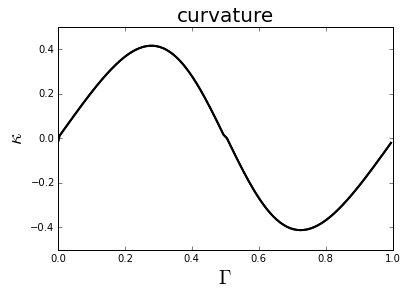
\includegraphics[width=2.5in,height=1.5in]{curvatureT0.png}
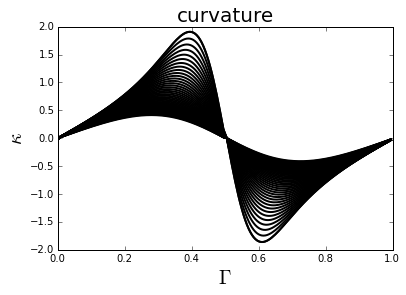
\includegraphics[width=2.5in,height=1.5in]{curvatureT04.png}
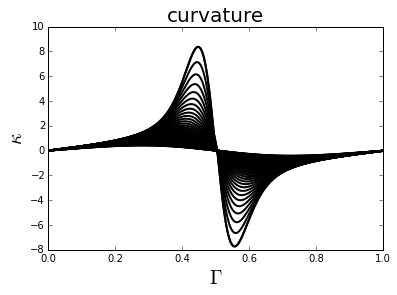
\includegraphics[width=2.5in,height=1.5in]{curvatureT054.png}
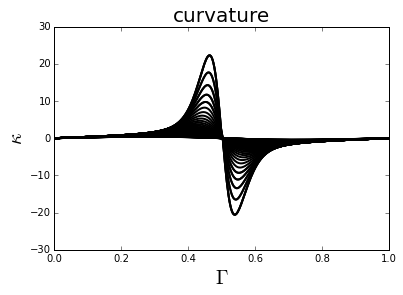
\includegraphics[width=2.5in,height=1.5in]{curvatureT06.png}
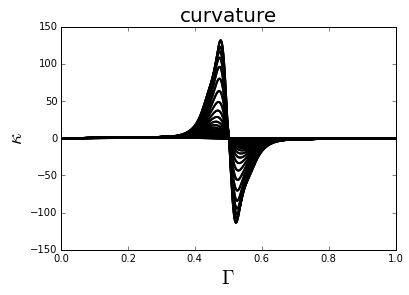
\includegraphics[width=2.5in,height=1.5in]{curvatureT07.png}


\caption{curvature withN=400 , $\delta=0.1$ , at  $T=0,0.4,0.54.6,0.7$}
\end{minipage}
\quad
\begin{minipage}[b]{0.45\linewidth}
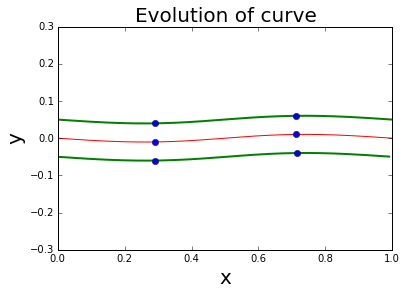
\includegraphics[width=2.5in,height=1.5in]{curveT0.png}
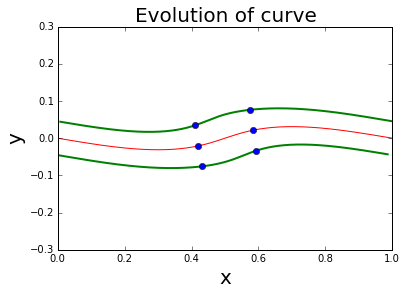
\includegraphics[width=2.5in,height=1.5in]{curveT04.png}
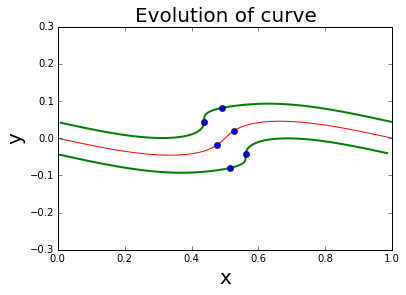
\includegraphics[width=2.5in,height=1.5in]{curveT054.png}
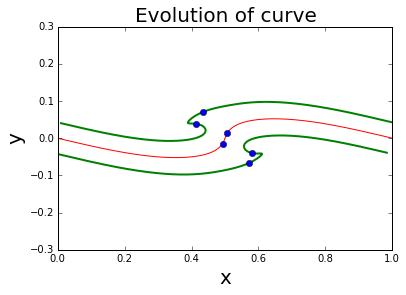
\includegraphics[width=2.5in,height=1.5in]{curveT06.png}
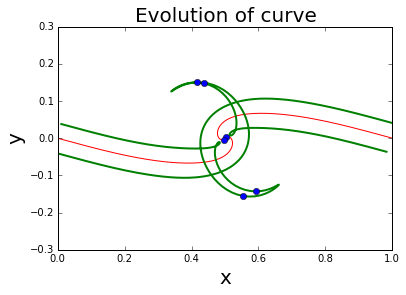
\includegraphics[width=2.5in,height=1.5in]{curveT07.png}
\caption{curve withN=400 , $\delta=0.1$ , at  $T=0,0.4,0.54.6,0.7$}

\end{minipage}
\end{figure}
\begin{figure}[ht]
\centering
\begin{minipage}[b]{0.45\linewidth}
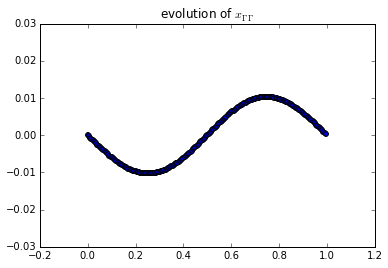
\includegraphics[width=3in,height=2in]{xppT0.png}


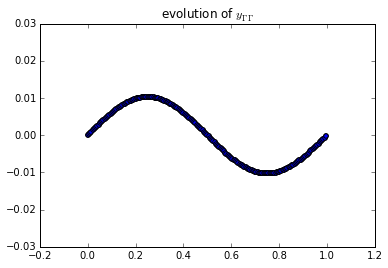
\includegraphics[width=3in,height=2in]{yppT0.png}

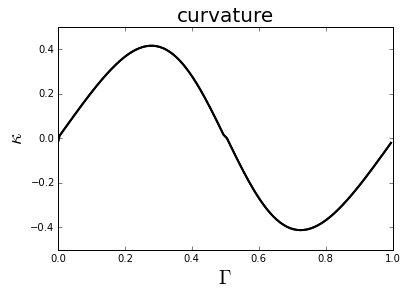
\includegraphics[width=3in,height=2in]{curvatureT0.png}
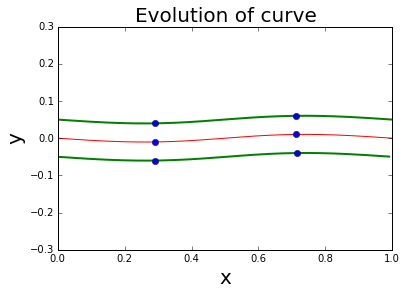
\includegraphics[width=3in,height=2in]{curveT0.png}
\caption{N=400 , $\delta=0.1$ , T=0}
\end{minipage}
\quad
\begin{minipage}[b]{0.45\linewidth}
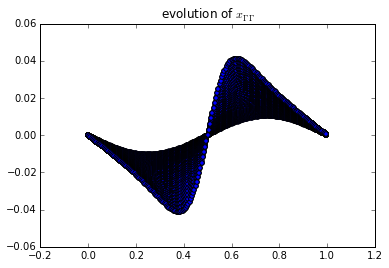
\includegraphics[width=3in,height=2in]{xppT04.png}

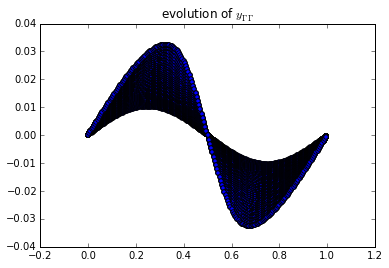
\includegraphics[width=3in,height=2in]{yppT04.png}

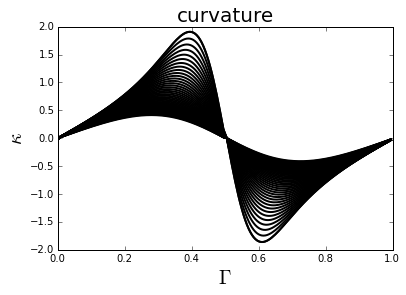
\includegraphics[width=3in,height=2in]{curvatureT04.png}
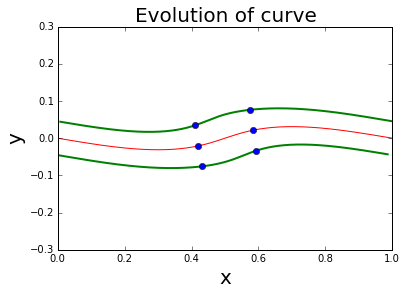
\includegraphics[width=3in,height=2in]{curveT04.png}
\caption{N=400 , $\delta=0.1$ , T=0.4}
\end{minipage}
\end{figure}


\begin{figure}[ht]
\centering
\begin{minipage}[b]{0.45\linewidth}
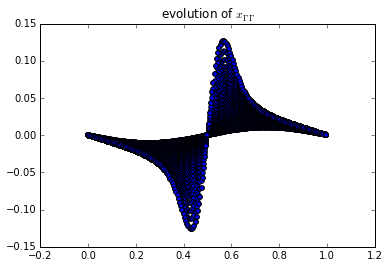
\includegraphics[width=3in,height=2in]{xppT054.png}

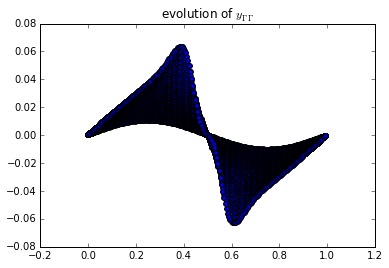
\includegraphics[width=3in,height=2in]{yppT054.png}

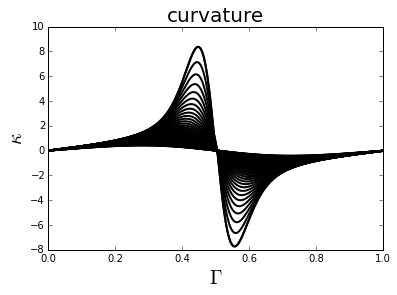
\includegraphics[width=3in,height=2in]{curvatureT054.png}
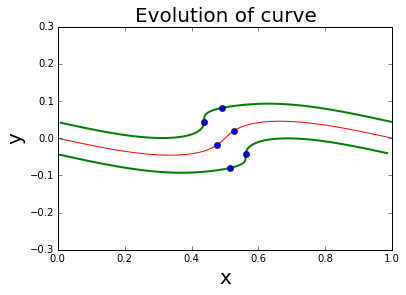
\includegraphics[width=3in,height=2in]{curveT054.png}
\caption{N=400 , $\delta=0.1$ , T=0.54}
\end{minipage}
\quad
\begin{minipage}[b]{0.45\linewidth}
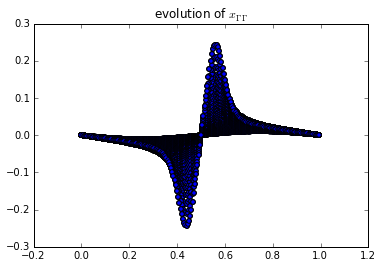
\includegraphics[width=3in,height=2in]{xppT06.png}
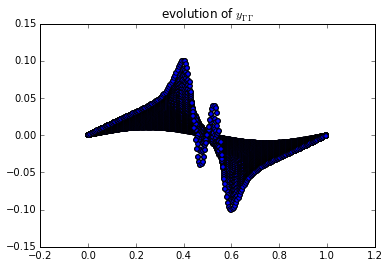
\includegraphics[width=3in,height=2in]{yppT06.png}
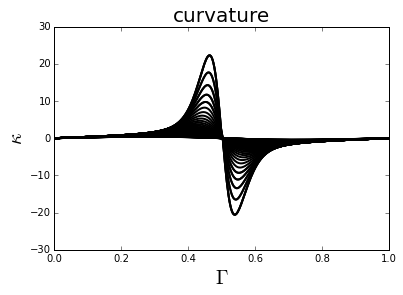
\includegraphics[width=3in,height=2in]{curvatureT06.png}
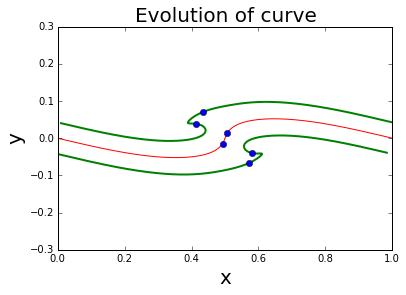
\includegraphics[width=3in,height=2in]{curveT06.png}
\caption{N=400 , $\delta=0.1$ , T=0.6}

\end{minipage}
\end{figure}


\begin{figure}[ht]
\centering
\begin{minipage}[b]{0.45\linewidth}
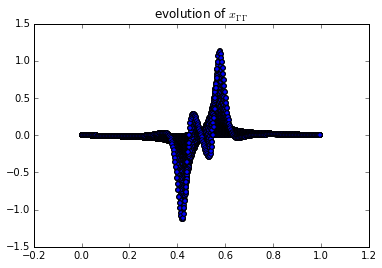
\includegraphics[width=3in,height=2in]{xppT07.png}
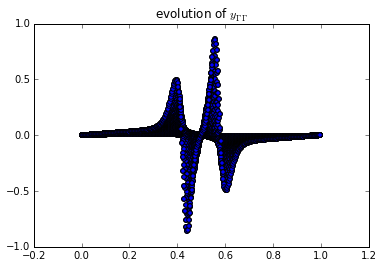
\includegraphics[width=3in,height=2in]{yppT07.png}
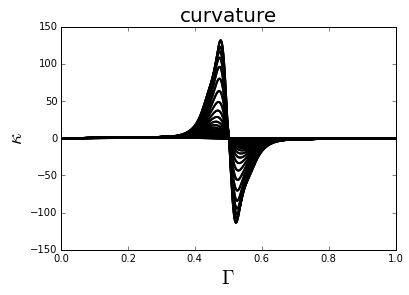
\includegraphics[width=3in,height=2in]{curvatureT07.png}
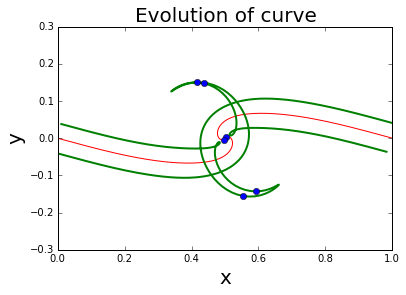
\includegraphics[width=3in,height=2in]{curveT07.png}
\caption{N=400 , $\delta=0.1$ , T=0.7}

\end{minipage}
\quad
\end{figure}



\end{document}